\documentclass[tikz,border=6pt]{standalone}
\usepackage{tikz}
\usetikzlibrary{arrows.meta}
\definecolor{nebula}{HTML}{6366F1}
\definecolor{spark}{HTML}{14B8A6}
\definecolor{ink}{HTML}{334155}
\begin{document}
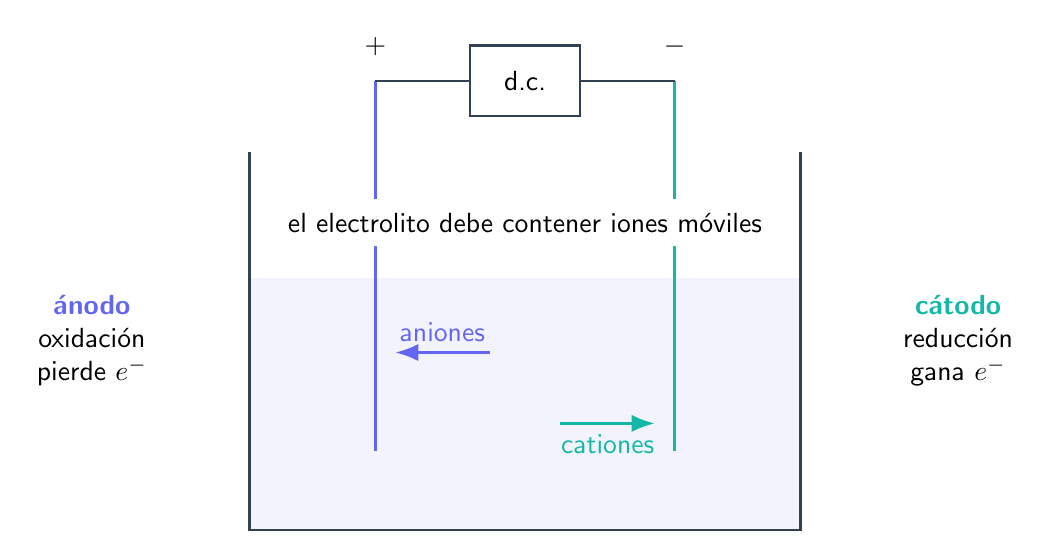
\begin{tikzpicture}[font=\sffamily,>=Latex]
  \fill[nebula!8] (0,0) rectangle (7,3.2);
  \draw[thick,ink] (0,4.8)--(0,0)--(7,0)--(7,4.8);
  \draw[very thick,nebula] (1.6,1)--(1.6,5.7);
  \draw[very thick,spark] (5.4,1)--(5.4,5.7);
  \draw[thick,ink] (1.6,5.7)--(2.8,5.7);
  \draw[thick,ink] (4.2,5.7)--(5.4,5.7);
  \draw[thick,ink] (2.8,5.25) rectangle (4.2,6.15);
  \node at (3.5,5.7) {d.c.};
  \node[above] at (1.6,5.9) {$+$};
  \node[above] at (5.4,5.9) {$-$};
  \draw[->,very thick,nebula] (3.05,2.25)--(1.85,2.25) node[midway,above] {aniones};
  \draw[->,very thick,spark] (3.95,1.35)--(5.15,1.35) node[midway,below] {cationes};
  \node[align=center] at (-2.0,2.4) {\textcolor{nebula}{\bfseries \'anodo}\\oxidaci\'on\\pierde $e^-$};
  \node[align=center] at (9.0,2.4) {\textcolor{spark}{\bfseries c\'atodo}\\reducci\'on\\gana $e^-$};
  \node[fill=white,rounded corners=4pt,inner sep=5pt] at (3.5,3.9) {el electrolito debe contener iones m\'oviles};
\end{tikzpicture}
\end{document}
